Рассмотрим и произведём вычисление трудоёмкости для классического алгоритма и алгоритма Винограда для умножения матриц $ А[MxN] $ и $ B[NxQ] $

\section{Классический алгоритм умножения}
Данный алгоритм непосредственно использует вышеприведённую формулу. Для вычисления каждого элемента матрицы С 
совершается циклический обход k элементов из таблиц А и B.

Схема алгоритма приведена на рисунке 2.1.
\begin{figure}[h]
	\begin{center}
		{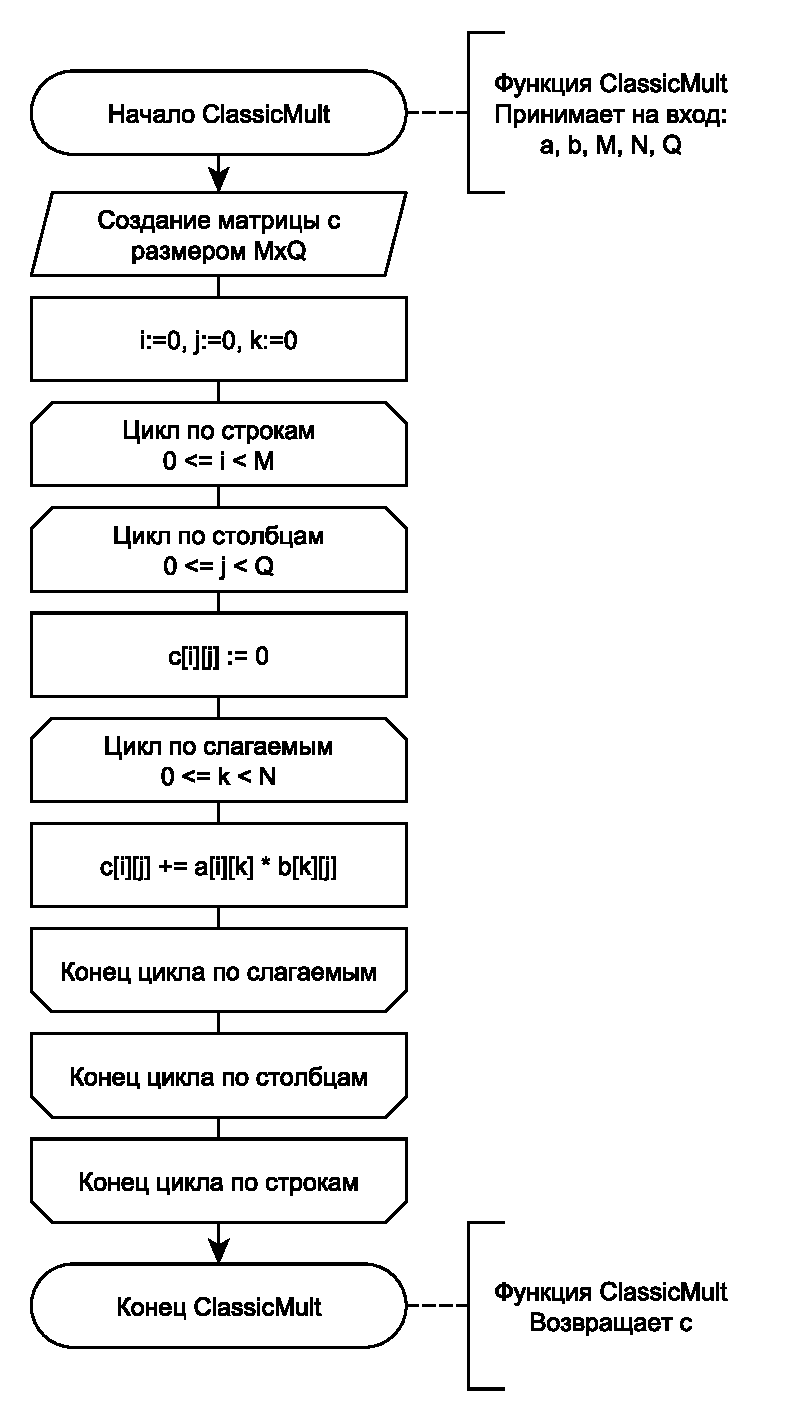
\includegraphics[scale = 0.8]{Classic}}
		\caption{Классический алгоритм умножения матриц}
	\end{center}
\end{figure}

% //////////////
\section{Алгоритм Винограда}
Цель алгоритма заключается в сокращении доли умножений в самом трудоёмком участке кода. Основная идея заключается в следующем. 

Пусть $ u, v $ - элементы матриц А, B соотв., участвующие в вычислении значения элемента матрицы C. Тогда данный элемент вычисляется как 
$ u_{1}v_{1} + u_{2}v_{2} + u_{3}v_{3} + u_{4}v_{4}$.
Такое выражение можно представить как 
$ (u_{1} + v_{2})(v_{1} + u_{2}) + (u_{3} + v_{4})(v_{3} + u_{4}) - u_{1}u_{2} - u_{3}u_{4} - v_{1}v_{2} - v_{3}v_{3})$. В этом выражении вычитаемые можно вычислить однократно и применить их для всех столбцов и строк, где они используются. Таким образом можно снизить трудоёмкость алгоритма за счёт снижения количества операций.

В случае, если матрица нечётный размер N, требуется производить дополнительные вычисления для крайних строк и столбцов. Таким образом, алгоритм наиболее эффективен в случае матриц, у которых N является чётным.

Схема алгоритма приведена на рисунках 2.2. и 2.3.
\begin{figure}[h]
	\begin{center}
		{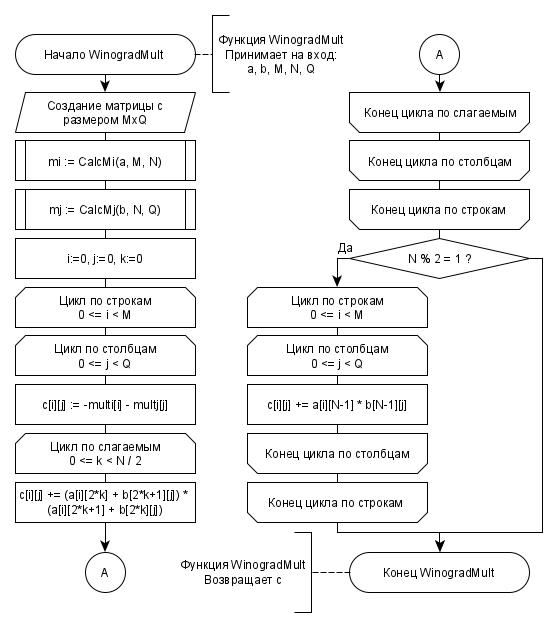
\includegraphics[scale = 0.8]{Winograd1}}
		\caption{Алгоритм Винограда}
	\end{center}
\end{figure}
\begin{figure}[h]
	\begin{center}
		{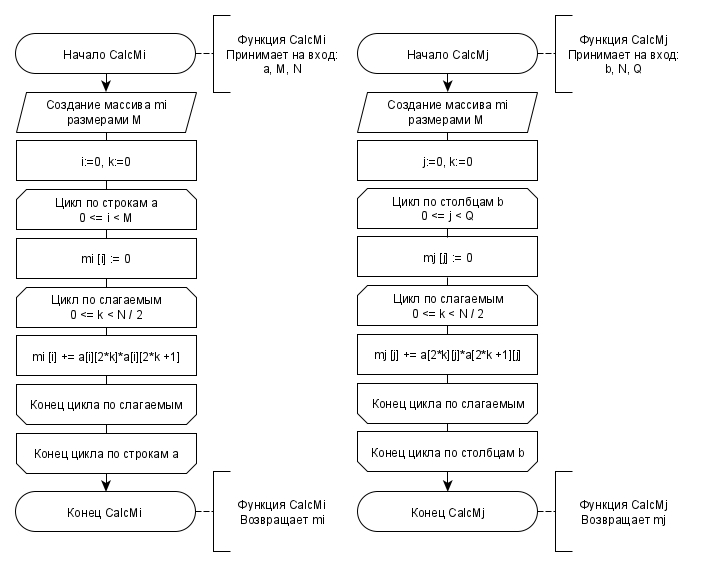
\includegraphics[scale = 0.7]{Winograd2}}
		\caption{Алгоритм Винограда, функции вычисления вспомогательных массивов}
	\end{center}
\end{figure}


% //////////////
\section{Требования к программному обеспечению}
Для полноценной проверки и оценки алгоритмов необходимо выполнить следующее.
\begin{enumerate}
	\item Обеспечить возможность консольного ввода двух матриц и выбора алгоритма для умножения. Программа должна вывести результирующую матрцу.
	\item Реализовать функцию замера процессорного времени, затраченного функцией. Для этого также создать возможность ввода размера матрицы, на которых будет выполнен замер.
\end{enumerate}

% //////////////
\section{Заготовки тестов}
При проверке алгоритмов необходимо будет использовать следующие классы тестов:
\begin{itemize}
	\item матрицы размером 1х1;
	\item две или одна пустая матрица;
	\item квадратные матрицы;
	\item чётный и нечётный размер N;
\end{itemize}



